%!TEX root = /Users/domaubert/Documents/Lectures/cosmolog/cosmo_main.tex

\chapter{Le Fond Diffus Cosmologique}

Le fond diffus cosmologique constitue la pierre angulaire de la cosmologie actuelle et se présente comme l'un des objets astrophysique le mieux connu et le plus étudié. C'est la conjonction d'une excellente compréhension théorique de cet objet avec l'avalanche de données de grande qualité qui a contribué à installer le fond diffus comme l'un des plus grands succès de la cosmologie.

Le fond diffus cosmologique est communément appelé CMB (pour \textit{cosmic microwave background}) et est constitué des photons "libérés" lors du processus de dernière diffusion. Ce processus a opéré 380 000 ans après le Big Bang et ces photons sont toujours détectable aujourd'hui car présent en grande quantité. Ils sont les reliques d'un époque où l'équilibre matière-rayonnement régnait et présentent une distribution spectrale de corps noir. Ce corps noir possède une température caractéristique d'environ 3K. Il se caractérise également par une intensité sur le ciel qui est uniforme à un très grand niveau de précision. Une étude détaillé de ce rayonnement fait ressortir des fluctuations qui trace la distribution de matière à l'époque de son émission, donnant ainsi accès à une vue sans égal sur le cosmos à ces époques reculées.

\section{Recombinaison}
Si l'on se place après la fin de la nucléosynthèse primordiale ($t>3$ minutes), protons, photons et électrons sont en interaction via 2 types de réactions, la recombinaison et la diffusion Thompson:
\begin{eqnarray}
p + e^- &\leftrightarrow& H+ \gamma\label{e:rec}\\
\gamma +e^- &\leftrightarrow& \gamma +e^- 
\end{eqnarray}
Ces 2 couplages vont disparaître de façon simultanée sous l'effet de la baisse de la densité d'électrons (ou de protons libres) cosmique. On définit la fraction d'ionisation $x$ de la façon suivante:
\begin{equation}
x=\frac{n_p}{n_p+n_H}
\end{equation} 
qui vaut 1 lorsque que le gaz cosmique est complètement ionisé et 0 lorsqu'il est complètement neutre. Notons qu'en raison de la neutralité électrique, la densité de protons libres $n_p$ est égale à la densité d'électrons libres $n_e$. De même, le nombre d'atomes d'hydrogène (crée par l'assemblage d'un proton et d'un électron) est donné par $n_H=(1-x) (n_p+n_H)$. 

L'équation de recombinaison peut être équilibrée via les potentiels chimiques $\mu_p+ \mu_e =\mu_H$ et on rappelle que pour chaque espèce son abondance $n_i$ est donnée par:
\begin{equation}
n_i=g_ie^{\frac{\mu_i}{k_BT}}\left(\frac{m_i k_B T}{2\pi\hbar^2}\right)^{3/2}e^{-\frac{m_i c^2}{k_B T}}.
\end{equation}
On obtient alors l'équation décrivant l'évolution temporelle de la fraction ionisée:
\begin{equation}
\frac{1-x}{x^2}=n_B \frac{g_H}{g_e g_p} \left(\frac{k_B T}{2\pi\hbar^2}\right)^{-3/2} m_e^{-3/2} e^{\frac{\chi}{k_B T}},
\end{equation}
où $n_B=n_p + n_H$ désigne la densité de baryons et $\chi=13.6$ eV est l'énergie de liaison de l'atome d'hydrogène. Notons également que la densité de baryon peut s'écrire en fonction du nombre de photons $n_B=\eta n_\gamma\sim T^3$ et l'équation de l'état d'ionisation peut s'écrire:
\begin{equation}
\frac{1-x}{x^2}=A \eta \left(\frac{k_B T}{m_e c^2}\right)^{3/2}e^{\frac{\chi}{k_B T}}
\label{e:recomb}
\end{equation}
où $A$ est un pré-facteur fonction notamment des facteurs de dégénérescence. Notons que le terme de droite de l'équation \ref{e:recomb} ne dépend que du temps, par conséquent elle se résume à une équation du second degré sur $x$ à un instant donné. On rappelle que cette évolution manifeste \textit{un déplacement de l'équilibre} vers  la droite de l'équation \ref{e:rec}.
\begin{figure}[htbp]
	\centering
		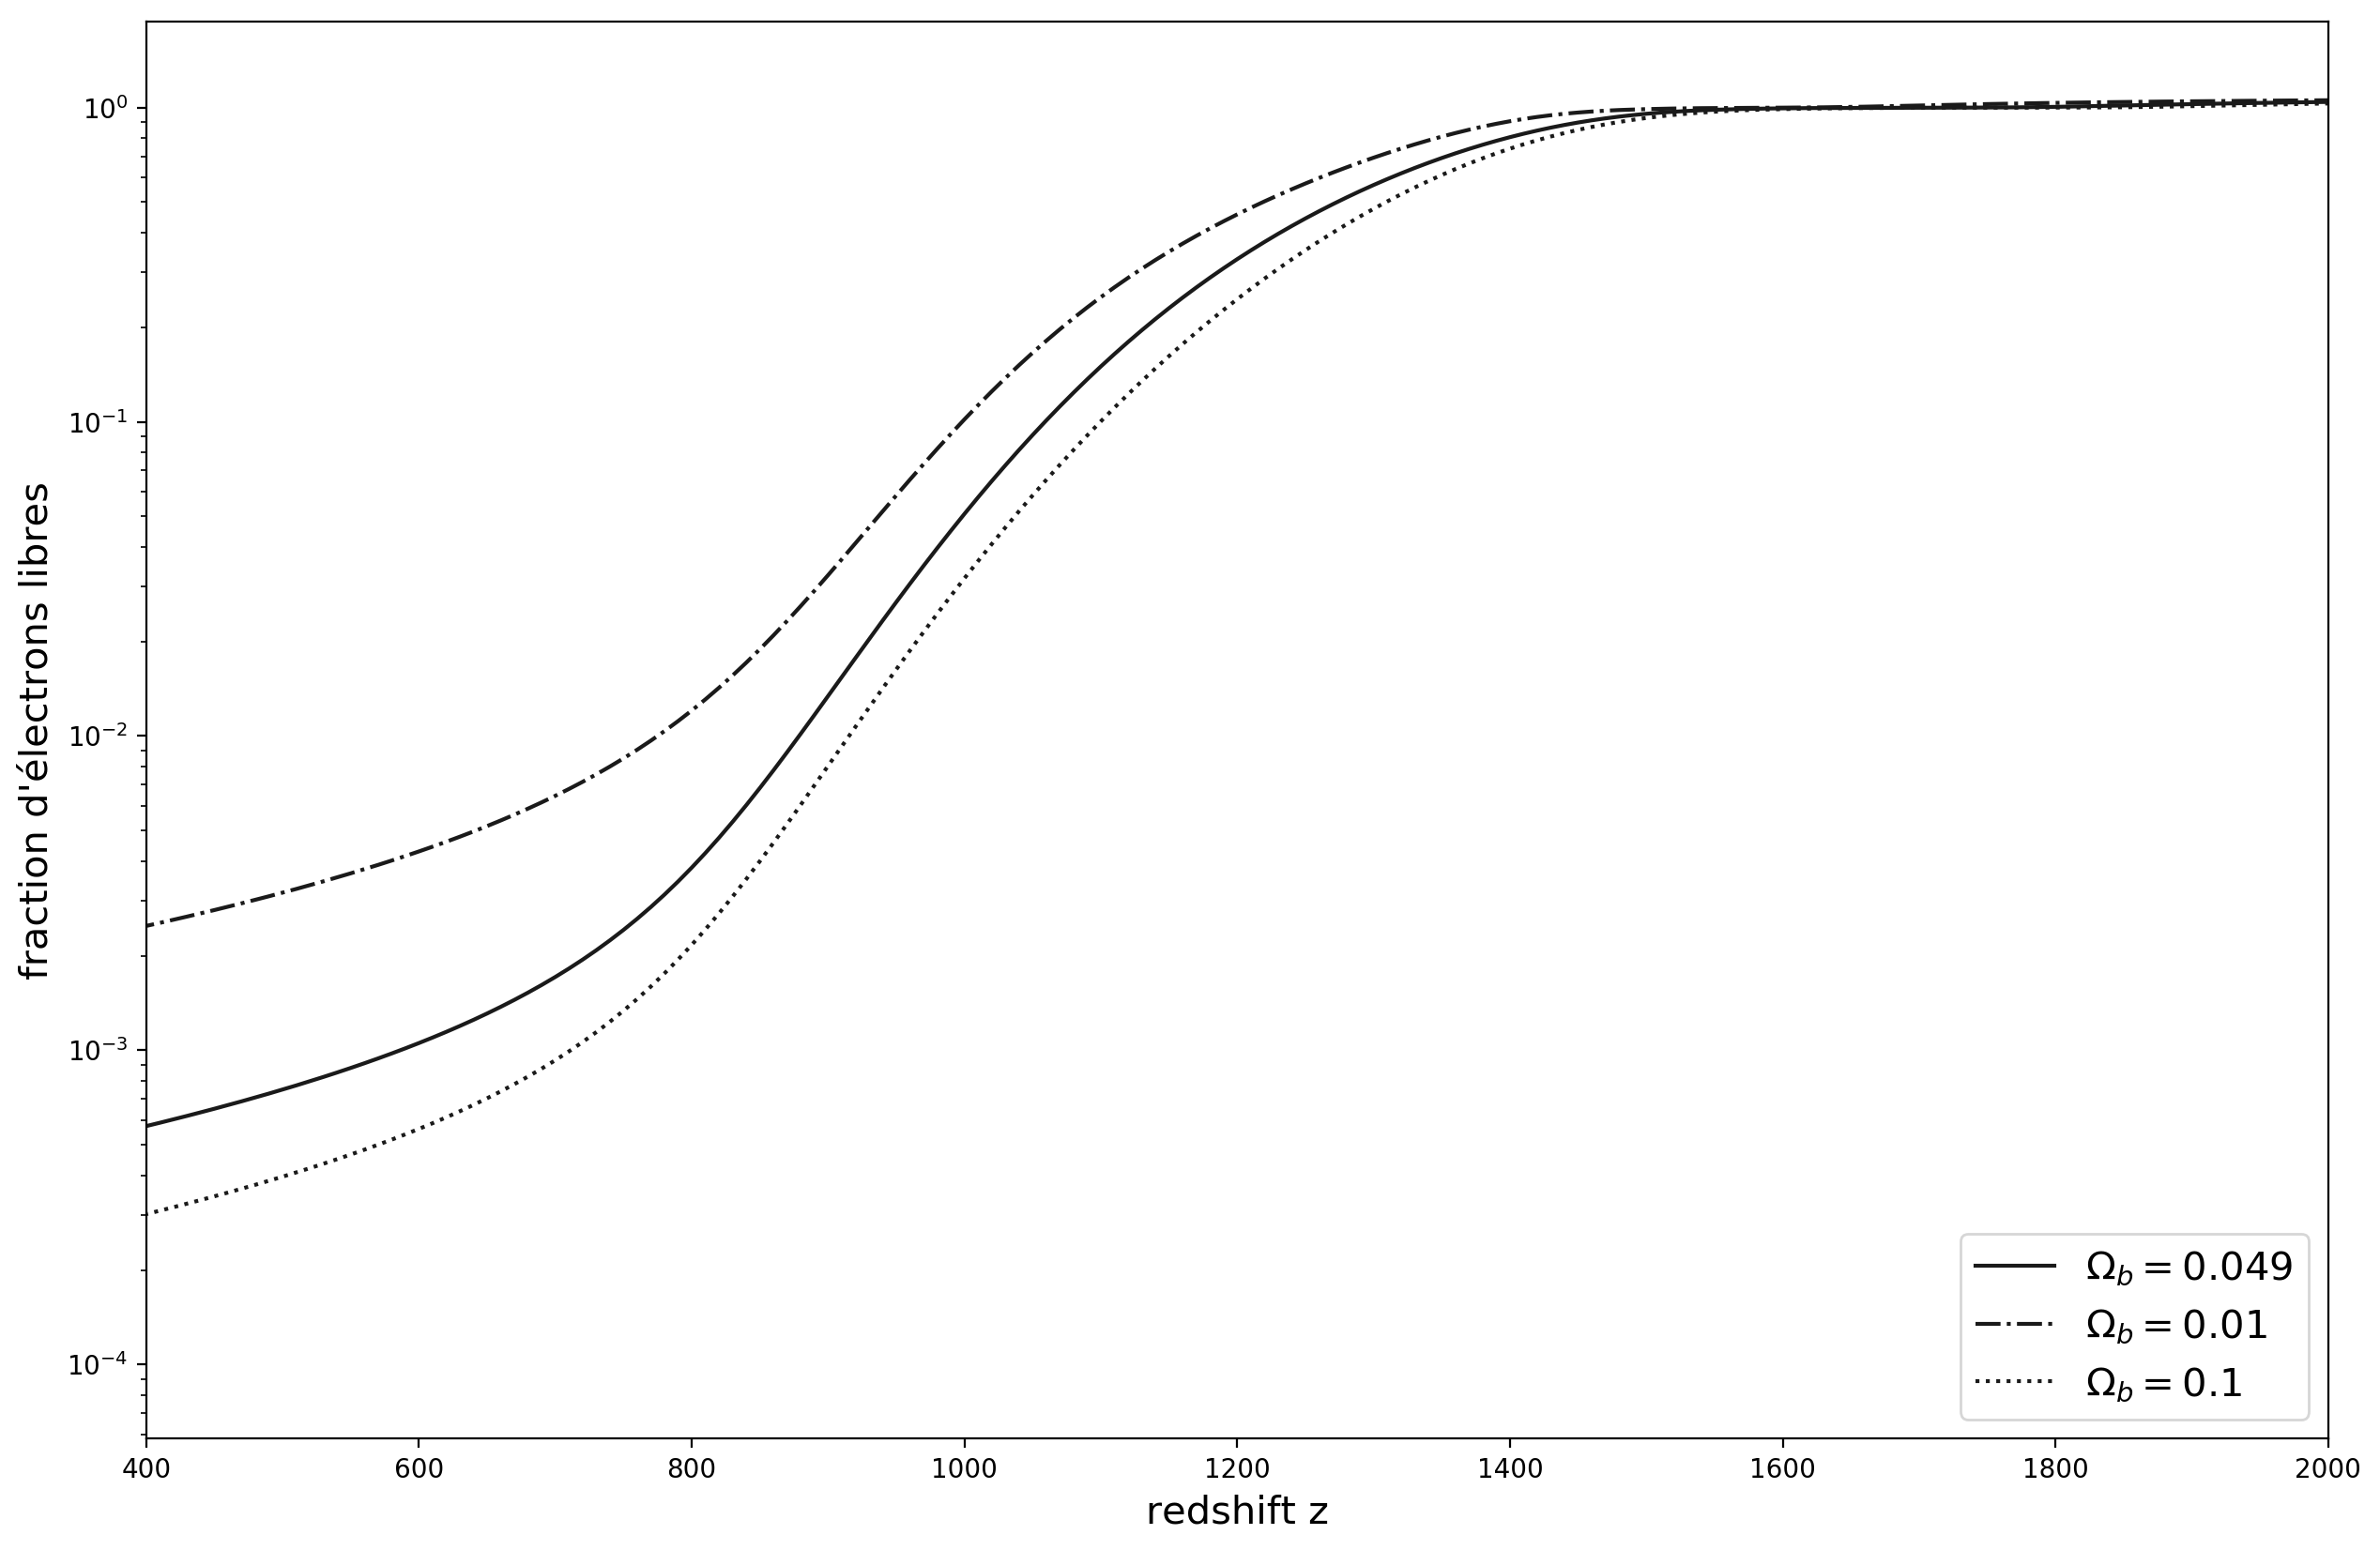
\includegraphics[height=10cm]{figs/recom.png}
		\caption{Evolution temporelle de fraction d'ionisation pour trois valeur de $\Omega_b$.}
	\label{f:recomb}
\end{figure}

La figure \ref{f:recomb} présente l'évolution de la fraction ionisée pour différente valeurs de $\Omega_b$. . Dans tous les cas l'Univers voit la quantité d'atomes ionisés divisée d'un facteur 100-1000 entre z=1500 et z=1000, correspondant à un âge d'Univers t=380 000 ans. On peut constater que ce processus opère plutôt tardivement: l'époque correspondant à l'énergie caractéristique $\chi=$13.6 eV s'est mise en place à $t=180$ ans. De manière analogue au deutérium bottleneck, c'est la grande quantité de photons (par rapport au nombre de baryons) qui empêche une mise en place plus rapide. Si l'on examine la figure \ref{f:recomb} plus en détail on constate d'une part qu'une plus faible densité de baryon ($\Omega_b$ plus faible) conduit à une mise en place moins efficace de la recombinaison. Elle opère plus tardivement et est moins complète dans un Univers moins riche en baryons.

\section{Surface de dernière diffusion}

\paragraph{Fin de la diffusion Thompson} La baisse de la densité électronique qui accompagne la formation d'atomes neutres conduit également à réduire l'efficacité de la diffusion Thompson. Dans un environnement riche en électrons libres, la diffusion force un court libre parcours moyen des photons et empêche le rayonnement de se propager sur de longues distances: c'est la marque d'un Univers opaque, dans lequel l'information ne peut provenir de régions lointaines.  Toutefois lorsque $x\sim 0.01\%$, la diffusion gèle, et se produit alors la \textit{dernière diffusion} à un redshift z=1100. A partir de cet instant, le rayonnement n'interagit plus avec les électrons et de fait se découple de la matière~: ce rayonnement peut dorénavant se propager librement et est détecté aujourd'hui sous la forme du CMB. Notons pour finir que la baisse de la densité électronique va également conduire au gel des réactions de recombinaison vers z=1100, avec un ionisation résiduelle de l'ordre de 0.01\%.

\paragraph{surface de dernière diffusion}
A partir de $z=1100$ les photons du fond diffus vont pouvoir se propager librement et de façon essentiellement rectiligne. Les photons du fond diffus qui nous parviennent aujourd'hui sont donc issus de toutes les régions du celle distantes de telle manière à ce que le rayonnement mette 13.8 milliards d'années à nous parvenir. L'ensemble de ces régions définit une coquille, centrée sur l'observateur et de distance de parcours lumineux égale à l'âge de l'Univers. Cette coquille possède une faible épaisseur, correspondant à la durée qu'aura mis la diffusion Thompson à geler, comparable à la durée qu'à mis la recombinaison à se mettre en place ($\Delta z\sim 100$). Vu depuis l'observateur, cette coquille apparaît donc comme une surface sphérique vue depuis l'intérieur, \textit{la surface de dernière diffusion}. Les régions au delà de cette surface de dernière diffusion nous sont inaccessibles par l'intermédiaire des photons, puisque ces derniers n'emporte que l'information de la dernière diffusion~: les régions au delà de cette sphère sont opaques à toute observation et les régions en deçà (à l'intérieur) de cette sphère constitue l'Univers observable de l'observateur placé en son centre.

Rappelons que ces photons sont ultra-dominant en nombre, avec par exemple un rapport baryon/photon $\eta\sim6e-10$. Cela a plusieurs conséquences: d'une part cela signifie qu'aucun processus astrophysique n'est en mesure de faire disparaître ce rayonnement et il est de fait toujours mesurable aujourd'hui. D'autre part cette domination est telle que l'impression même de signatures de processus astrophysique entre z=1100 et aujourd'hui ne peut se faire qu'à des niveaux très faible. Par conséquent ce rayonnement possède toujours un spectre de corps noir (décalé vers le rouge) même si il n'est plus en situation d'équilibre avec la matière. De même les éventuelles marques des propriétés de l'Univers âgé de 380 000 ans s'y trouve toujours. L'observation de la surface de dernière diffusion est donc une fenêtre incomparable sur l'état du cosmos à ces époques lointaines.

\section{Corps noir cosmologique}
Le fond diffus cosmologique est issu d'une époque où matière et rayonnement étaient couplés et par conséquent possédait à ces époques reculées un spectre de corps noir. La densité volumique de photons dans l'intervalle $[\nu,\nu+d\nu]$ est donné par:
\begin{equation}
n(\nu)d\nu=\frac{8\pi}{c^3}\frac{\nu^2d\nu}{e^{h\nu/k_BT}-1}.
\end{equation}
Comme indiqué précédemment, la surabondance de ces photons est telle que ce signal a conservé les caractéristique d'un tel corps noir, même dans un régime de faible couplage entre matière et rayonnement. Aujourd'hui la température de ce 'corps noir' est mesurée avec une très grande précision (voir aussi la figure \ref{f:bb}):
\begin{equation}
T_0=2.7255\pm0.0006 K.
\end{equation}
\begin{figure}[htbp]
	\centering
		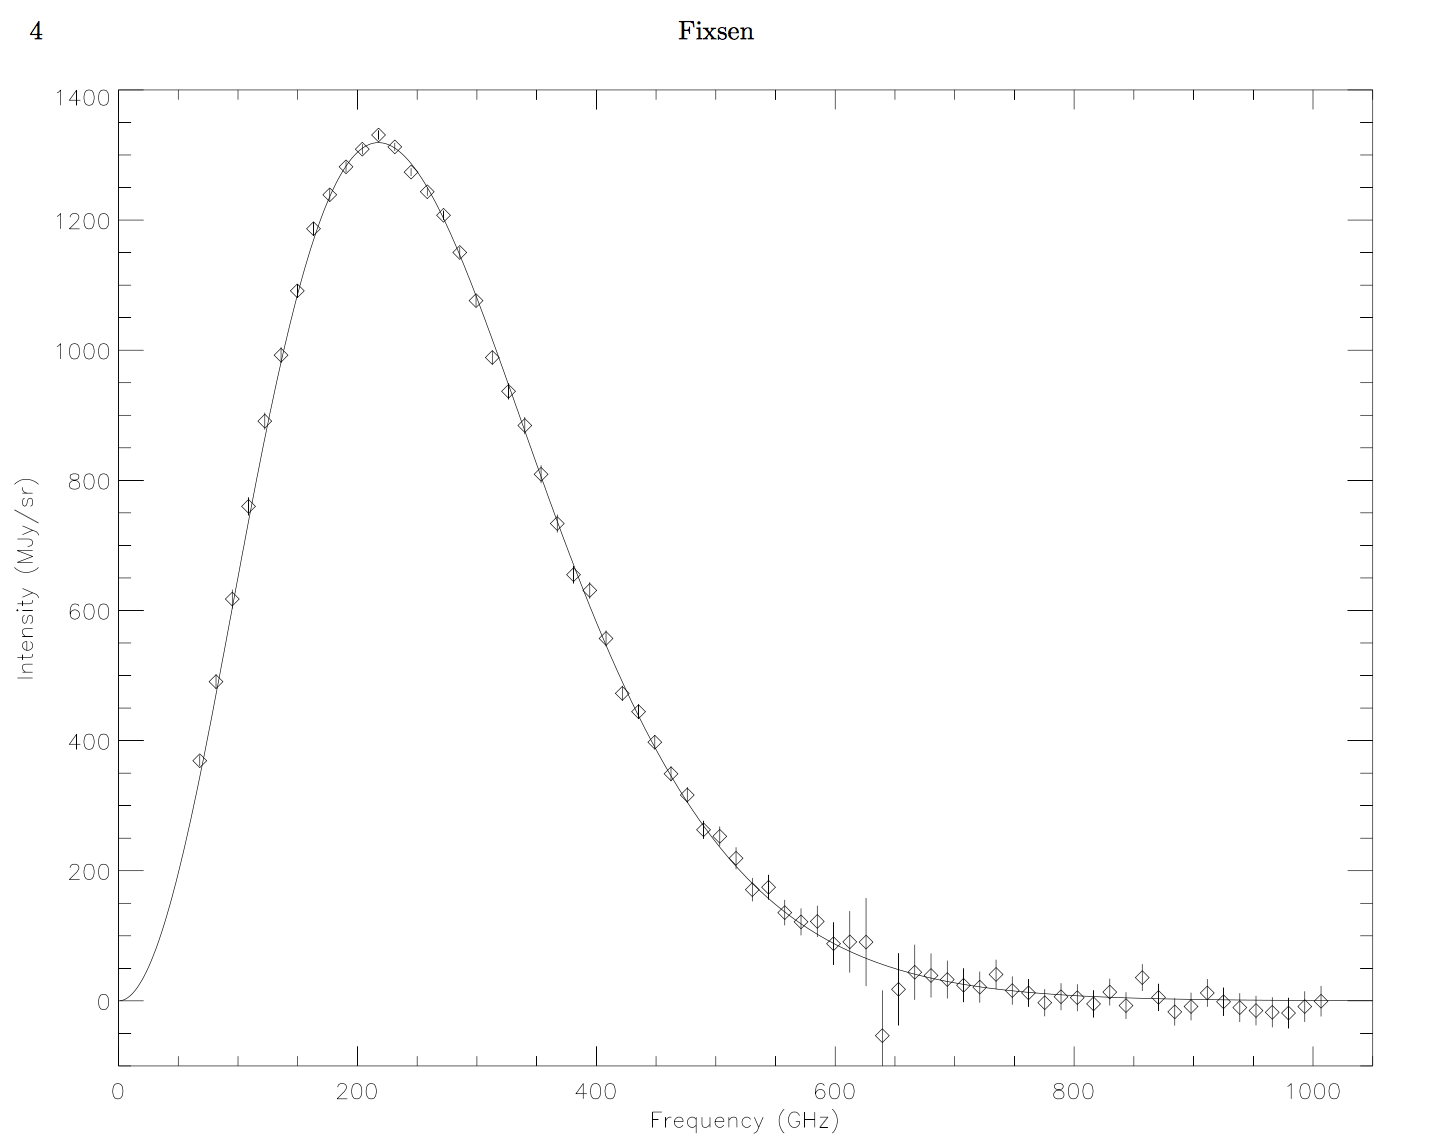
\includegraphics[height=10cm]{figs/bb.png}
		\caption{Le spectre du fond diffus cosmologique: les symboles représentent les mesures de l'instrument FIRAS, la ligne le spectre de corps noir pour une température de $T_0=2.725$K. Figure extraite de Fixsen 2009.}
	\label{f:bb}
\end{figure}
Ce spectre va conserver sa forme, malgré le redshift des photons concernés et malgré la modification de leurs fréquences selon:
\begin{equation}
\nu(a)=\frac{\nu_0}{a}.
\end{equation}
Dans un volume de contrôle de volume $V=V_0a^3$ et dans un intervalle de fréquence $d\nu=d\nu_0/a$, le nombre de photon doit rester identique quel que soit l'instant considéré:
\begin{equation}
\frac{\nu^2d\nu}{e^{h\nu/k_BT}-1}V=\frac{\nu_0^2d\nu_0}{e^{h\nu_0/k_BT_0}-1}V_0,
\end{equation}
qui ne peut être satisfait que si la température caractéristique du corps noir suit la relation :
\begin{equation}
T=\frac{T_0}{a}=T_0(1+z)
\end{equation}
que nous avions déjà établi. On remarque ainsi que la recombinaison opérant à $z\sim1100$, la température du gaz de photon cosmique était proche des 3300 K.

\section{Anisotropies du CMB}
Le fond diffus est représentatif d'un Univers jeune (t=380 000 ans) et donc très proche de l'homogénéité parfaite. Par conséquent sa mesure fait apparaître une très grande stabilité du signal sur tout le ciel, sans fluctuations de température détectable jusqu'à des niveaux de 0.001 K. Au delà, commence toutefois à apparaître des anisotropies dans le signal~: celles-ci sont essentiellement générées par la physique des baryons à l'œuvre au moment de la recombinaison et par des processus astrophysiques qui affecte le rayonnement au cours de son vol jusqu'à l'observateur. L'étude de ces anisotropies est extrêmement riche d'informations pour la physique fondamentale, la cosmologie et l'astrophysique. Notons que nous allons nous concentrer sur les fluctuations de température et implicitement le mot "fluctuation" ou "signal" désigne ce type de donnée. Il existe également des études en \textit{polarisation} que nous n'aborderons que très rapidement en fin de chapitre.

\begin{figure}[htbp]
	\centering
		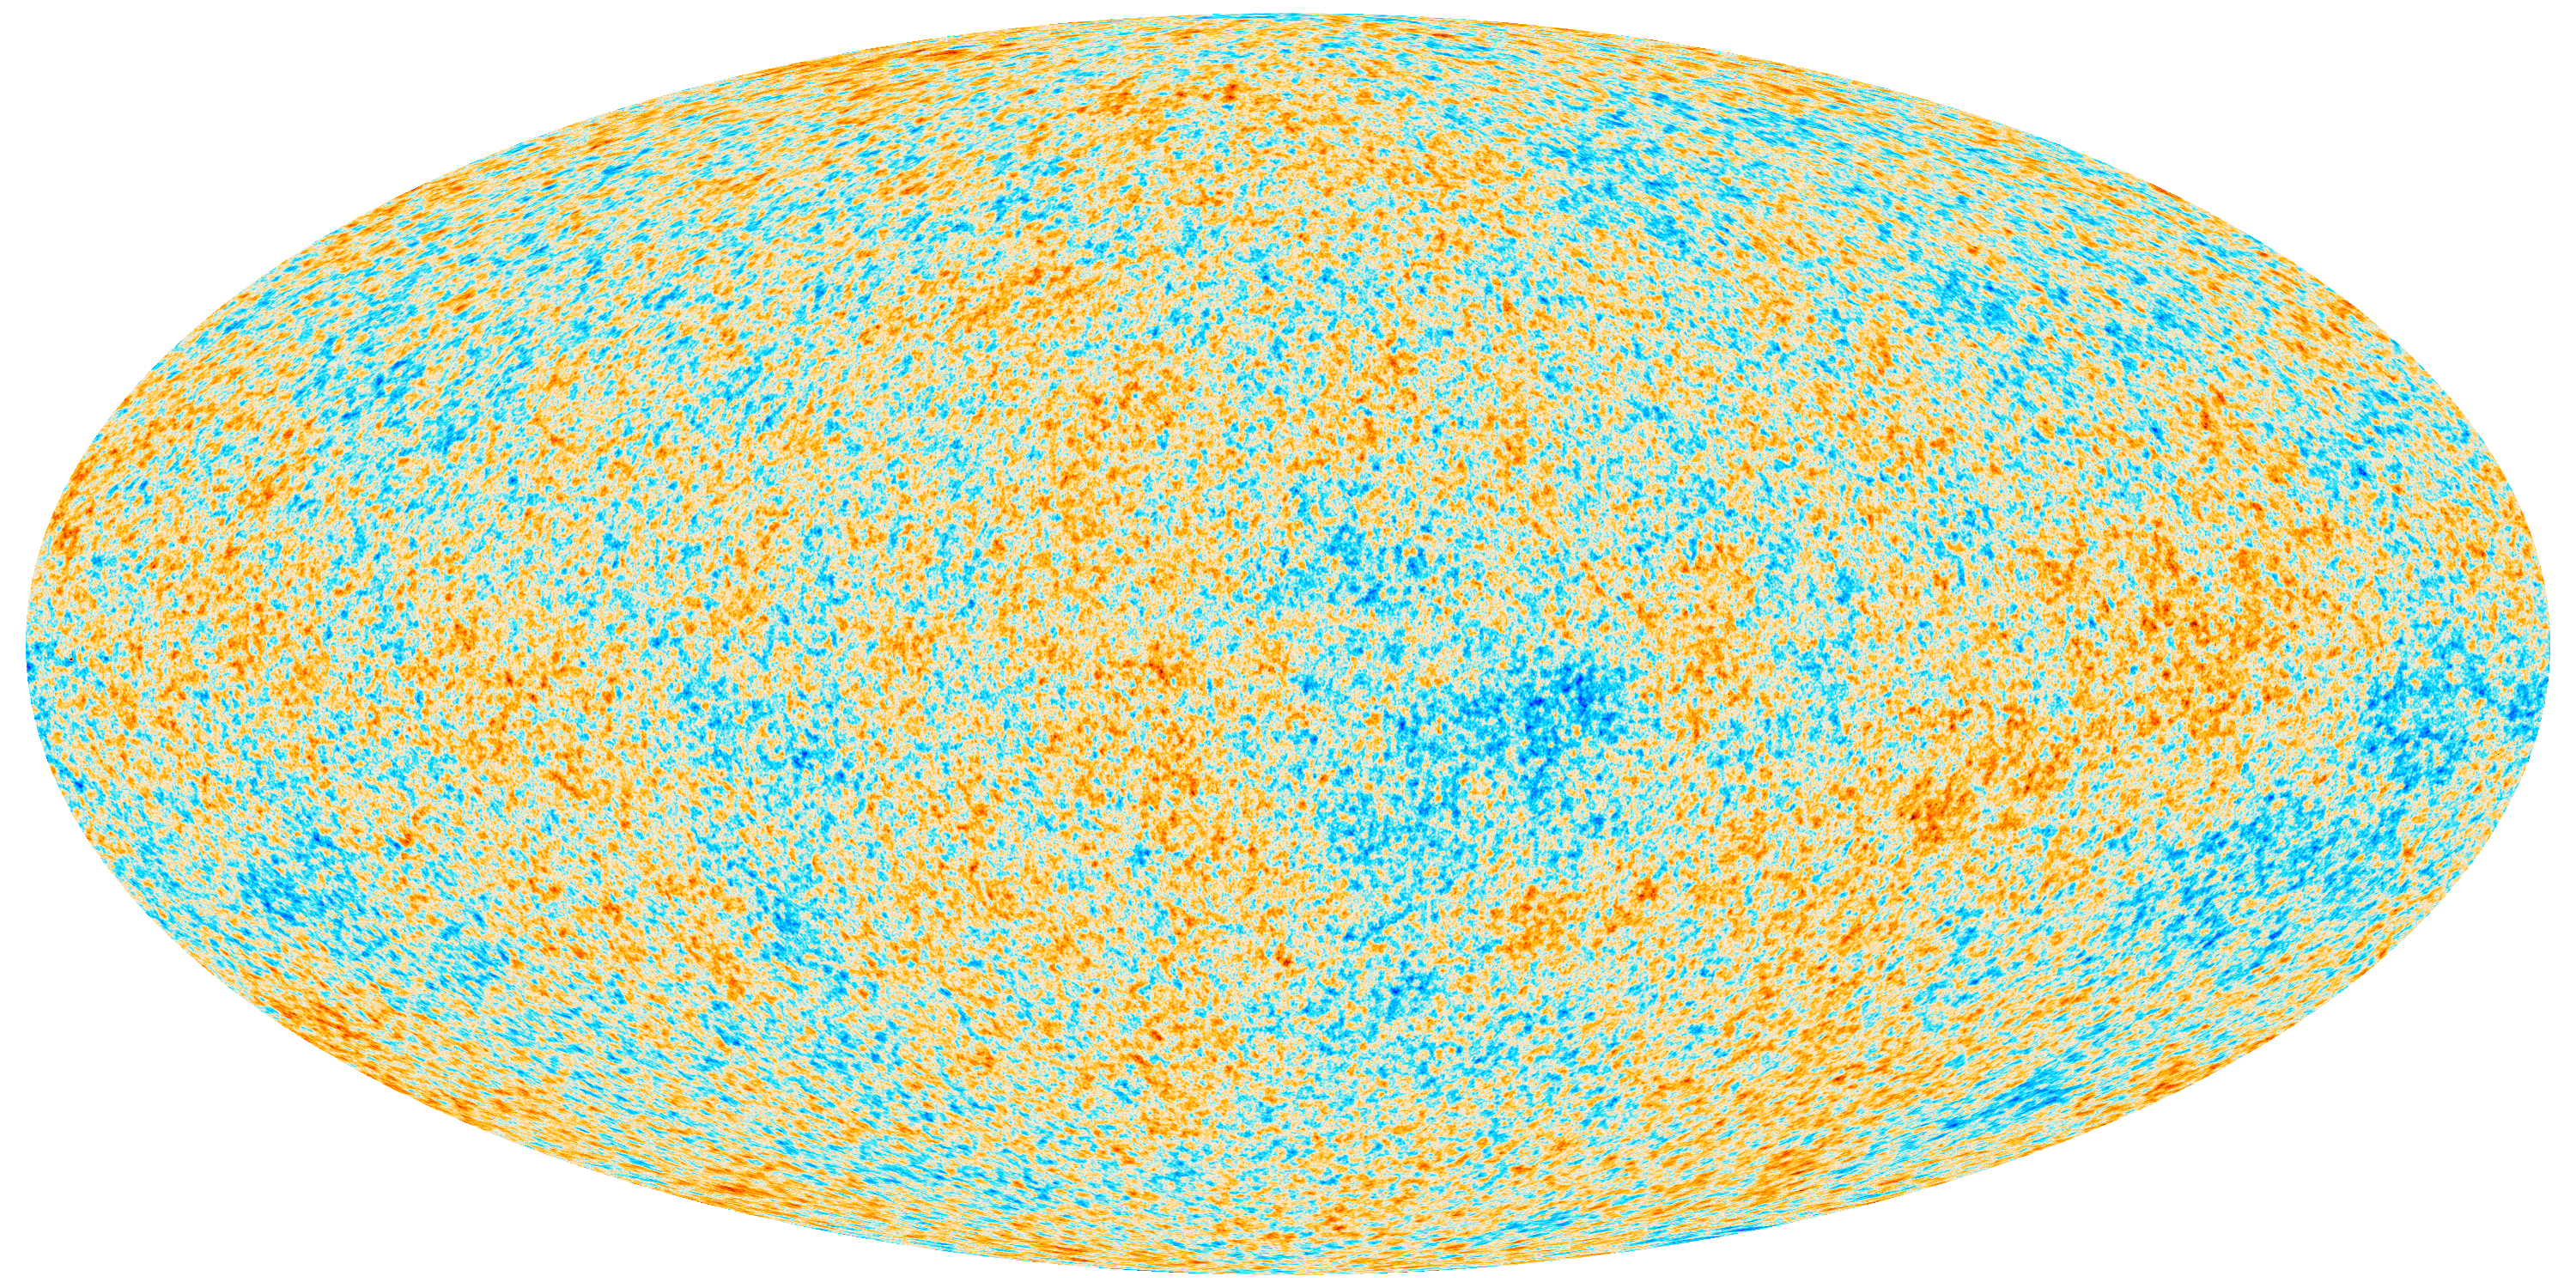
\includegraphics[height=6cm]{figs/planck2015.png}
		\caption{La carte des anisotropies du fond diffus obtenue par la mission européenne \textit{Planck}. Les zones jaunes sont plus chaudes que les zones bleues. Le niveau des fluctuations représentées est de l'ordre de 0.001\%.}
	\label{f:planckmap}
\end{figure}

\subsection{Principe de l'analyse des anisotropies du CMB}
Dans cette section, nous allons exposer rapidement les grands principes de l'analyse du signal du fond diffus. Le CMB se manifeste pour l'observateur comme un signal sur tout le ciel, généralement sous la forme d'une carte de température $\delta T(\theta,\phi)$, mesurée dans un repère sphérique. Afin de pouvoir extraire de l'information de ce type de données, l'on raisonne généralement sur la transformée de Fourier de ce signal. Cette opération permet d'une part de séparer les contributions des différentes échelles angulaires. D'autre part, nous verrons que la théorie qui permet de prédire les propriétés de ces fluctuations se fait naturellement dans l'espace de Fourier, où les différentes échelles angulaires évoluent de façon découplées en très bonne approximation.  Dans un espace sphérique, les opérations de transformées de Fourier s'effectue via la base des harmoniques sphériques $Y_{\ell,m}(\theta,\phi)$ et la carte de températures se décompose de la façon suivante:
\begin{equation}
\delta T(\theta,\phi)= \sum_{\ell=0}^{\infty}\sum_{m=-\ell}^{\ell} a_{\ell,m} Y_{\ell,m}(\theta,\phi),
\end{equation}
où les coefficients (complexes) $a_{\ell,m}$ sont obtenus par projection de la carte sur la base vectorielle composée des harmoniques:
\begin{equation}
a_{\ell,m}=\int \int d\theta d\phi\sin \theta Y^*_{\ell,m}(\theta,\phi) \delta T(\theta,\phi).
\end{equation}
Les coefficients $a_{\ell,m}$ constituent ainsi la contribution de chaque harmonique à la carte de température.

\paragraph{Echelles angulaires}
 Les harmoniques sphériques sont les analogues des modes de Fourier sur la sphère, à savoir une base de sinus et cosinus adapté à une géométrie sphérique. Le coefficient $\ell$ trace l'échelle angulaire de l'harmonique qui possède ainsi une taille angulaire caractéristique $\theta\sim\pi/\ell$: on parle également de fréquence angulaire où les bas $\ell$ désigne les grandes échelles sur le ciel et les grands $\ell$ les petites échelles. Le coefficient $m$ peut varier entre $-\ell$ et $\ell$ et désigne les différentes orientations indépendantes pour chaque taille angulaire caractéristique: celle ci sont d'autant plus nombreuses que la fréquence angulaire est élevée. L'harmonique $\ell=0$ correspond au monopole, à savoir un signal uniforme sur toute la sphère et dont le coefficient $a_{00}$ renvoie directement à la moyenne sur tout le ciel. Les harmoniques $\ell=1$ sont des dipôles, avec un côté 'chaud' et un côté 'froid' diamétralement opposés.

\paragraph{Spectre de puissance}
\begin{figure}[htbp]
	\centering
		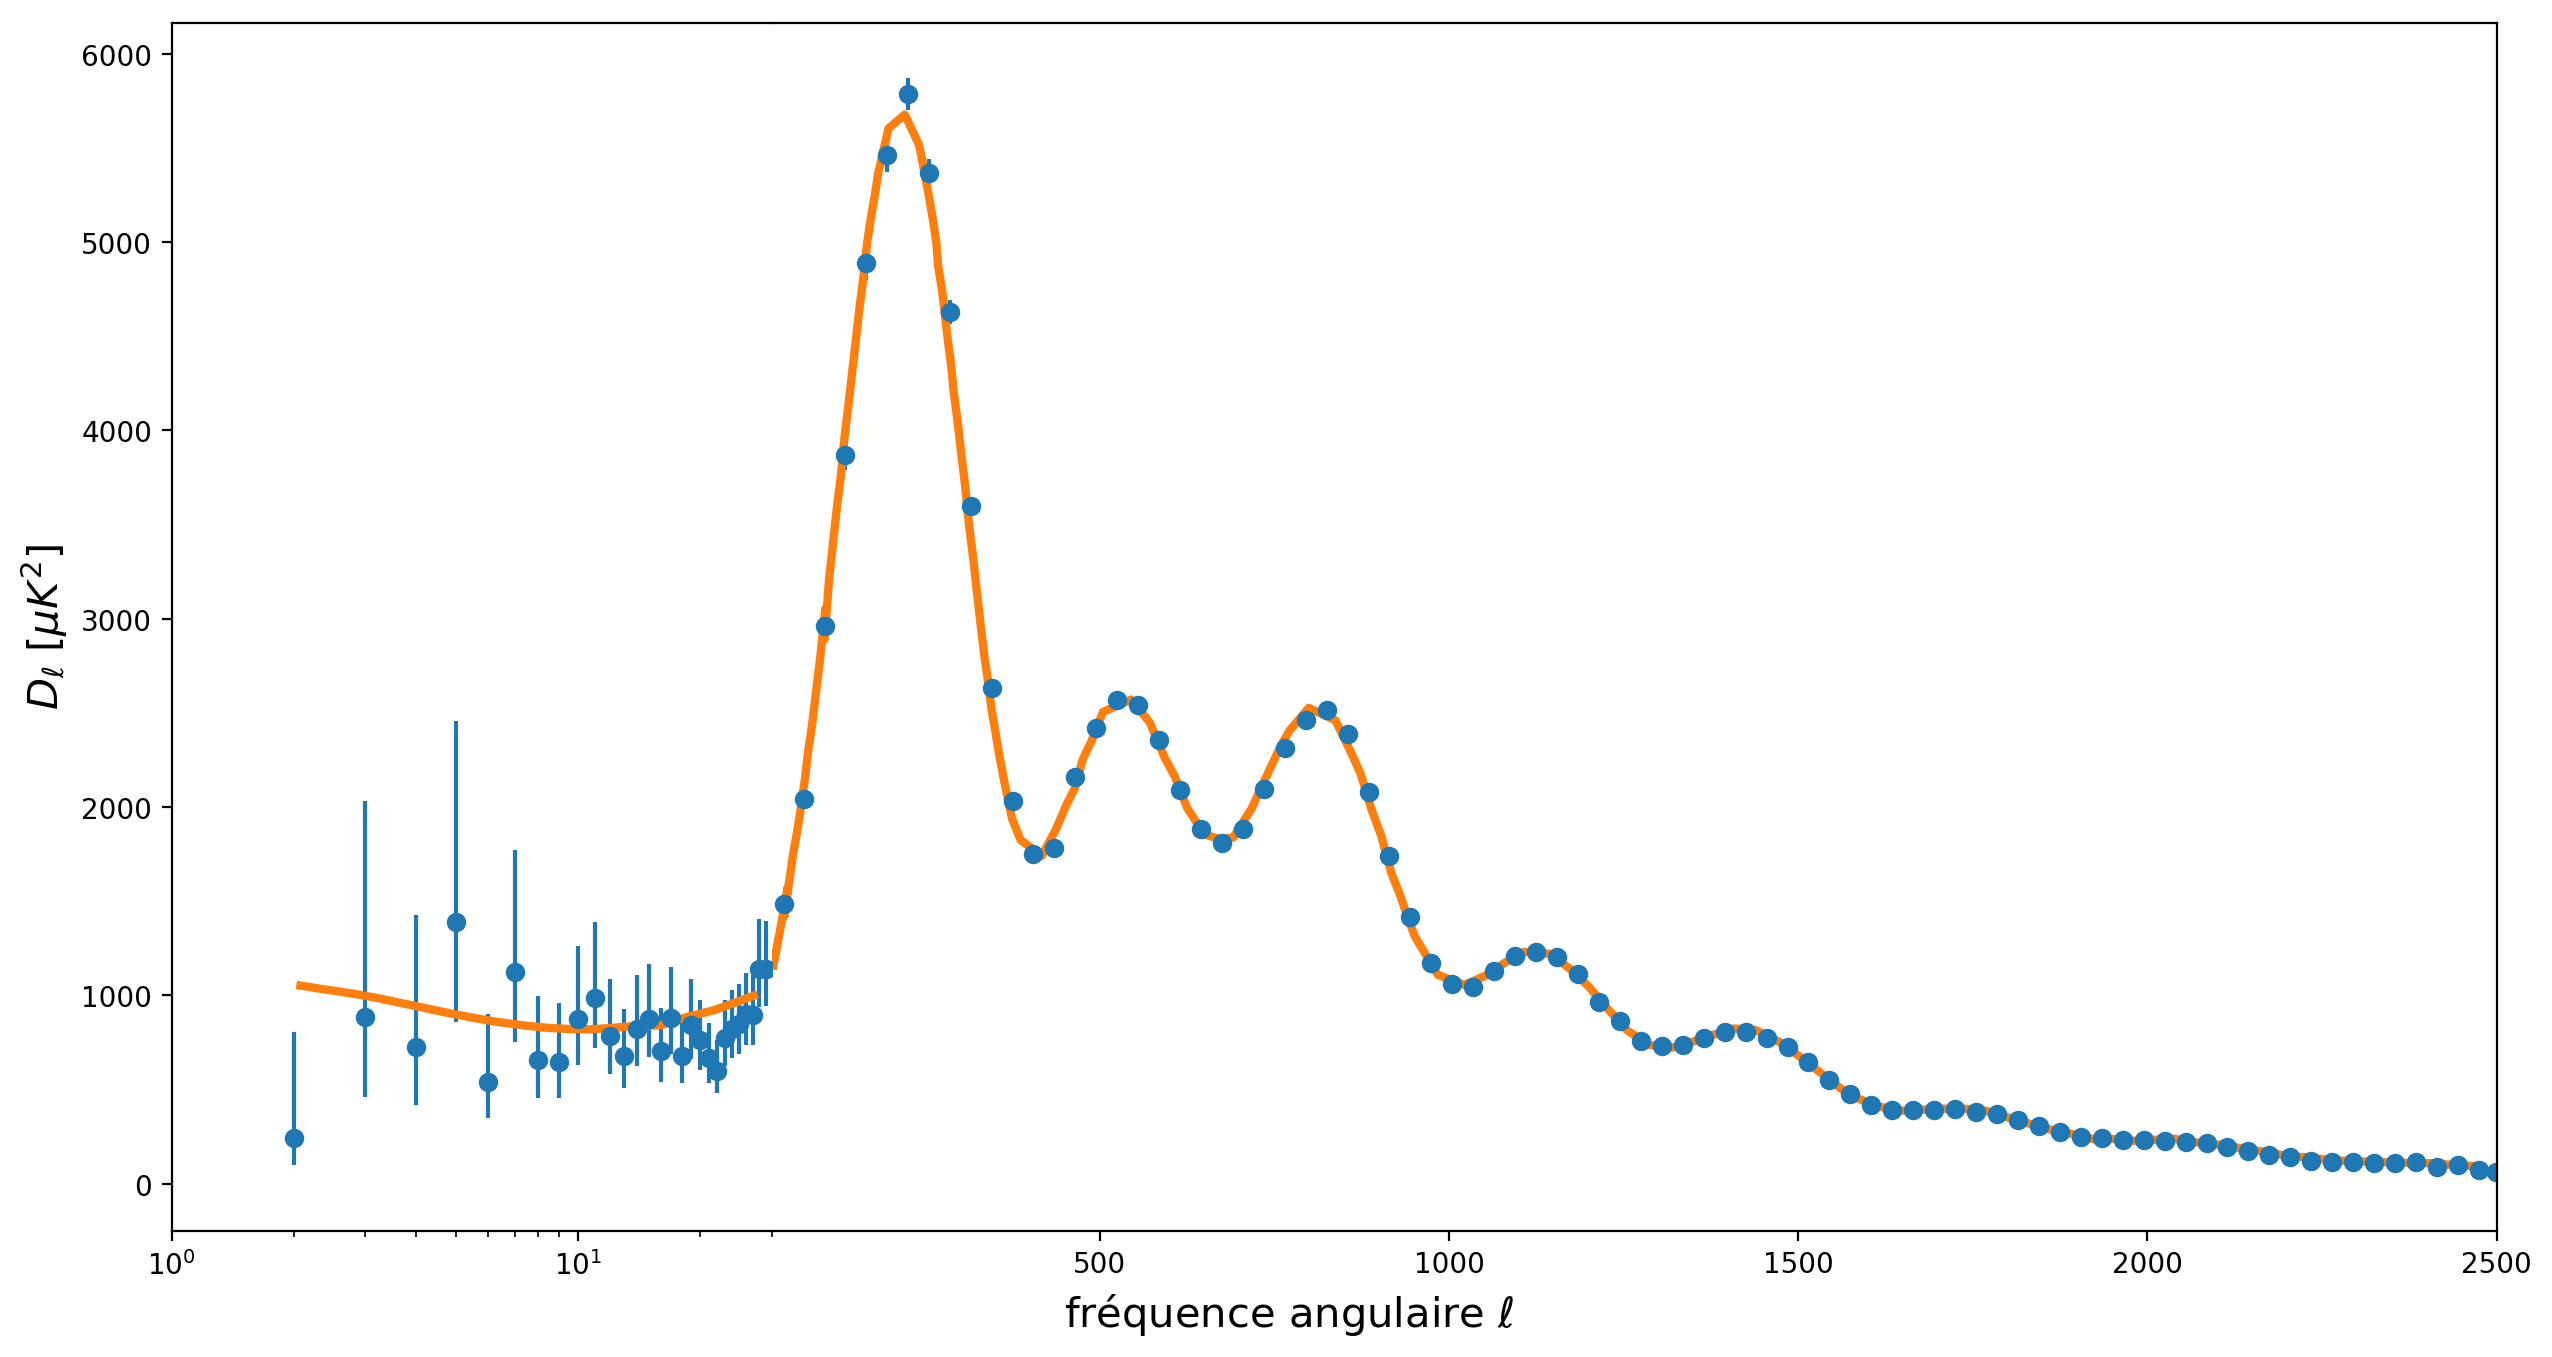
\includegraphics[height=8cm]{figs/cl2015.png}
		\caption{Le spectre de puissance des anisotropies du fond diffus cosmologique obtenu par \textit{Planck}. Le panneau supérieur représente $D_\ell=\ell(\ell+1)C_\ell$~: les points sont les données et la ligne représente le spectre prévu pour un modèle $\Lambda$CDM. Le panneau inférieur montre les résidus entre le modèle et les points de données.}
	\label{f:cl}
\end{figure}

Armé de la collection des coefficients $a_{\ell,m}$ d'une carte du ciel, on évalue les contributions relatives de chaque échelle par le spectre de puissance angulaire:
\begin{equation}
C_\ell=\langle |a_{\ell,m}|^2\rangle=\frac{1}{2\ell+1}\sum_{m=-\ell}^{\ell} |a_{\ell,m}|^2
\end{equation}
Ce faisant, on rassemble pour chaque échelle angulaire $\ell$ les contributions de toutes les orientations $m$ associées. Si toutes les directions sont à priori équivalentes et aucune n'est privilégiée, alors cette opération ne produit pas de perte d'information. C'est le cas du CMB, celui-ci étant à priori isotrope. D'autre part, une grande classe de modèles d'inflation prédisent que les fluctuations du fond diffus doivent appartenir à la classe des \textit{champs aléatoires gaussiens} qui sont entièrement définis par leur 'variance', ce qui est précisément la nature du spectre de puissance angulaire.

\subsection{Avant-plans}

Avant toute chose, il est important de réaliser qu'une carte brute du ciel aux longueurs d'ondes sondées par les missions CMB est soumise à une forte contamination par des avant-plans astrophysiques. Parmi ces avant-plans, le plus spectaculaire est sans contexte la Galaxie dont par exemple l'émission  par les poussières ou le rayonnement synchrotron empêchent d'accéder aux fluctuations du CMB en arrière plan. Ces avant-plans peuvent être ajustés, modélisés et pris en compte dans des modèles d'inversion, afin d'extraire le signal d'origine cosmologique des portions du ciel affectées. Notez que ces avant-plans sont également source de recherches dédiées, notamment à propos des propriétés des poussières dans la Voie Lactée.

\paragraph{Dipôle} Le premier niveau d'anisotropie est constitué par le dipôle du CMB. Il possède une amplitude de l'ordre de 3 mK et résulte du mouvement de l'observateur par rapport à la surface de dernière diffusion. Ce mouvement induit un effet Doppler, fonction de la vitesse de déplacement et qui fait apparaître des zones plus chaudes et plus froides que la moyenne, diamétralement opposées et alignées avec la direction de déplacement. Au premier ordre, la variation de température dans la direction du dipôle obéit à la relation:
\begin{equation}
\left(\frac{\Delta T}{T}\right)_\mathrm{dipole}\sim \frac{v}{c}
\end{equation}
et donne une valeur de vitesse de déplacement $v\sim 330$ km/s pour le barycentre du système solaire. Cette vitesse est la somme notamment de la vitesse de déplacement du Soleil dans la Galaxie et de la Galaxie dans le Groupe Local.

\subsection{Anisotropies Intrinsèques}
Les fluctuations de température du CMB tracent des fluctuations de densité de matière. Plusieurs modèles de couplage entre matière et rayonnement existent, mais un grand nombre d'évidences observationnelles pointent vers des fluctuations de type \textit{adiabatiques}. Dans ce mode de couplage, le rapport entre la densité de matière et celle de rayonnement reste constant y compris au sein des fluctuations locales : le fluide de matière ne dérive pas par rapport au fluide de photons. Dans ce cas le rapport des densités reste constant:
\begin{equation}
\frac{n}{n_\gamma}=\mathrm{cste}\rightarrow\frac{\delta n}{n}=\frac{\delta n_\gamma}{n_\gamma}
\end{equation}
Pour la matière, densité de matière et d'énergie sont directement reliées $\epsilon=n m c^2$ et
\begin{equation}
\frac{\delta n}{n}=\frac{\delta \epsilon}{\epsilon}.
\end{equation}
Pour les photons, nous avons déjà vu que $n_\gamma \sim T^3$ :
\begin{equation}
\frac{\delta n_\gamma}{n_\gamma}=3 \frac{\delta T}{T}.
\end{equation}
D'où il apparaît que les fluctuations de températures tracent les fluctuations de densité via:
\begin{equation}
\left(\frac{\delta T}{T}\right)_\mathrm{adiab}=\frac{1}{3}\frac{\delta n}{n}=\frac{1}{3}\frac{\delta \rho}{\rho}.
\end{equation}
Dans un régime de fluctuations adiabatiques, les régions plus chaudes (respectivement plus froides) que la moyenne correspondent aux régions les plus dense au même moment. 

Toutefois les fluctuations de densité produisent également des fluctuations de potentiel gravitationnel qui devront être gravie ou dévalées par les photons du fond diffus au moment de leur émission. Les photons en train de sortir d'un puit (correspondant à une surdensité) seront décalées vers le rouge (perte d'énergie) et ceux en train de dévaler un pic de potentiel (correspondant à une sous densité seront décalés vers le bleu (gain d'énergie). Cet effet se nomme \textit{effet Sachs-Wolf}:
\begin{equation}
\left(\frac{\delta T}{T}\right)_\mathrm{SW}=-\delta\phi
\end{equation}
où $\delta \phi$ est la fluctuation de potentiel. Par ailleurs on peut montrer que la variation de potentiel est liée à la fluctuation de densité via $\delta \rho/\rho=2\delta \phi$ ce qui implique que la variation de température \textit{totale} est donnée par :
\begin{equation}
\left(\frac{\delta T}{T}\right)_\mathrm{total}=\left(\frac{\delta T}{T}\right)_\mathrm{SW}+\left(\frac{\delta T}{T}\right)_\mathrm{adiab}=-\frac{1}{3}\delta \phi=-\frac{1}{6}\frac{\delta \rho}{\rho}
\end{equation}
Les points chaud du CMB correspondent à des régions sous-dense de l'Univers au moment de l'émission. La carte de température du CMB est donc une carte de la distribution de matière au même instant. Ces fluctuations se situent à des niveaux de 0.001\%, indiquant par la même que l'Univers était extrêmement homogène au moment de la recombinaison.

\paragraph{Grandes échelles} Reste à expliciter l'origine des fluctuations de densité qui conduisent aux fluctuations de températures. L'examen de la figure \ref{f:cl} permet de distinguer 2 régimes. Le premier régime correspond aux grandes échelles $\ell<30$: ces modes sont plus grands que l'Horizon au moment de la recombinaison et tracent les fluctuations les plus primordiales, dont on pense qu'elles sont issues d'une période inflationnaire présente aux tous premiers instants après le Big-Bang. L'étude de ces régions du spectre permet notamment de mesurer l'amplitude des fluctuations inflationnaire ainsi que le spectre de ces fluctuations. En particulier, les théories inflationnaires indiquent que le spectre de puissance tridimensionnel des fluctuations primordiales doit être invariant d'échelle et de la forme:
\begin{equation}
P(k)\sim k^{n_s}
\end{equation}
avec $n_s$ proche mais différent de 1. Les résultats de \textit{Planck 2015} indiquent que $n_s=0.968\pm0.006$ en accord avec ces théories.

\paragraph{Petites échelles} Au delà de $\ell\sim 30$, le spectre présente un ensemble de modes correspondant à des échelles caractéristiques et qui se manifestent sous forme de pics: on en dénombre 3 principaux suivis d'environs 6 pics d'amplitude décroissante. Ces pics indiquent l'existence d'échelles privilégiées dans la carte des fluctuations: ces échelles résultent d'ondes sonores se propageant dans le plasma au moment de la recombinaison. Ces ondes sonores sont appelées \textit{oscillations baryoniques acoustiques} (BAO en anglais) : leur production sera décrite en détail dans le chapitre dédié à la croissance des grandes structures. Ces oscillations se mettent en place pour des échelles sub-horizon d'où leur présence seulement aux petites échelles: la position du premier pic permet ainsi de tracer la taille sur le ciel de l'horizon sonore. Connaissant la taille \textit{intrinsèque} de cet horizon, la mesure de la taille apparente permet de déduire la géométrie du cosmos le long du parcours des photons ($\Omega_m+\Omega_\Lambda$), qui de fait apparaît comme plane à un bon niveau de précision. Les pics suivants tracent la taille des modes ayant effectué un nombre de battement de plus en plus important entre leur production et l'émission du fond diffus. En particulier leur hauteurs relatives permet de contraindre précisément le couplage entre la matière et le rayonnement et la force de rappel qui permet d'entretenir ces battements. Cette force de rappel est induite par la gravité crée par la matière et la mesure de l'entretien de ces battements permet de contraindre la quantité de matière totale ($\Omega_b$ et $\Omega_m$). 

L'une des grandes leçons apprise par l'étude du CMB est la constatation que $\Omega_m>\Omega_b$, en particulier la grande amplitude du 3ème pic (et des suivants) ne peut s'expliquer par une matière purement baryonique: elle nécessite une matière non couplée avec le rayonnement, en quantité significative, \textit{la matière noire}. En l'absence de matière noire, le couplage entre matière et rayonnement n'est pas suffisamment important pour garantir un entretien maximal des oscillations baryoniques. Ce couplage imparfait conduit à un amortissement de ces dernières au cours des battements successifs : les échelles les plus petites, celles-qui oscillent le plus rapidement voient donc leur amplitude décroître. Dans le spectre de puissance angulaire, ce la se manifeste par des pics d'amplitude de plus en plus faible pour les hautes fréquences angulaires : on parle d'amortissement Silk. Or l'amplitude du 3ème pic (et des suivants) est supérieure à celle attendue dans le cas d'un gaz purement baryonique, i.e. en présence uniquement de matière capable d'intéragir avec le rayonnement (qui fournit le support de pression). Cet excès d'amplitude peut s'expliquer si il existe une force de rappel gravitationnelle supplémentaire, créée par de la masse \textit{qui n'est pas sensible à ce couplage rayonnement matière imparfait}. 

Cette matière noire, pèse, entretient les BAOs et n'intéragit pas avec le rayonnement : si elle existe, elles nous est actuellement inconnue. On retrouve également trace d'un effet similaire dans la masse des amas de galaxies, dans la dynamique des galaxies et dans les effets de lentille gravitationnelle.

\subsection{Anisotropies secondaires}
En plus des anisotropies imprimées dans le plasma au moment de le recombinaison, il existe tout un ensemble d'anisotropies crées par différents processus qui affectent les photons du CMB le long de leur parcours entre la surface de dernière diffusion et leur réception. Nous n'en citerons que 3 ici.

\paragraph{La réionisation} 
La réionisation désigne l'époque à laquelle les premières sources de rayonnement ionisant apparaissent dans l'histoire du cosmos entre 400 millions et 1 milliard d'années après le Big-Bang. Ces sources (essentiellement les premières étoiles et quasars) vont ioniser à nouveau le gaz cosmique, dans un court laps de temps et vont produire une nuée d'électrons libres susceptibles d'interagir avec les photons du CMB par effet Thompson. Cette interaction va influer sur l'amplitude des fluctuations de température et affecter le spectre du CMB en polarisation aux grandes échelles. Cette interaction se mesure via la profondeur optique Thompson $\tau$:
\begin{equation}
\tau=\int_{z_\mathrm{rec}}^{0} c\sigma_t n_e(z)\frac{dt}{dz}dt
\end{equation}
qui est une mesure du nombre d'interactions entre un photon du CMB et les électrons de la réionisation. Notons que si la réionisation est précoce, la densité d'électrons $n_e$ est grande et $\tau$ est grand tandis que si elle est tardive, cette densité sera plus faible par simple dilution cosmologique conduisant à une faible valeur de $\tau$. Les mesures du CMB indiquent que la réionisation a eu lieu pour $z_\mathrm{reion}\sim8$, en désaccord léger avec les autres sondes astrophysiques du processus qui proposent une réionisation plus tardive avec $z_\mathrm{reion}\sim6$.

\paragraph{L'effet SZ des amas}
Les amas de galaxies sont les plus grandes structures viriélisées de l'Univers actuel. Ils ont été formés récemment $z\sim 1$ et contiennent typiquement plusieurs centaines ou milliers de galaxies pour des masses totales approchant les $10^{14}-10^{15} M_\odot$. La masse très importante de ces objets font que le gaz piégé dans leur puit de potentiel gravitationnel est chauffé à des températures de l'ordre du million de K: à ces températures le gaz devient un fort émetteur X et est l'objet de processus d'ionisation collisionnelle. De façon analogue à la réionisation, les amas constitues des ilots denses d'électrons libres avec lesquels les photons du CMB peuvent interagir à des redshifts $z\sim 1$. On parle d'effet Sunyaev-Zeldovich, qui produisent de légère distorsions du spectre du CMB, en redistribuant l'énergie des photons vers de plus hautes valeurs. Les amas de galaxies présents sur le ciel produisent ainsi des anisotropies localisées, permettant même la découverte de tels objets avant confirmation par des observations X par exemple.

\paragraph{Le lentillage gravitationnel cosmique}
Les grandes structures croisées par les photons du CMB au cours de leur parcours entre l'émission et leur réception vont modifier subtilement la distribution sur le ciel des anisotropies primaires par effet de lentille gravitationnelle. Une lentille résulte d'une déformation locale de la métrique par une lentille faite de matière (galaxie, amas, filaments, etc..) qui courbe la trajectoire des rayons lumineux et modifie donc l'apparence des sources d'arrière plan. Dans le cas du CMB, la lentille est constituée de toutes les grandes structures rencontrées au cours de l'histoire de l'Univers tandis que la source d'arrière plan est la source la plus reculée imaginable. Cet effet de lentille se manifeste essentiellement aux petites échelles et dans le spectre angulaire en polarisation, il nécessite donc des expériences CMB de grande résolution pour pouvoir être extrait. Il a récemment été mesuré par les expériences sol tels que le \textit{South Pole Telescope} ou dans l'espace par \textit{Planck}. Cette mesure est extrêmement importante car elle permet de mesurer de façon quasi indépendante les paramètres cosmologiques à partir de la croissance des grandes structures qui opère à des redshifts différents de la physique du CMB ($z\sim 2$). Elle permet une forte levée de dégénérescence des paramètres mesurés par les fluctuations de températures. Pour l'essentiel les paramètres contraints par le lentillage du CMB confirment les paramètres $\Lambda$CDM obtenus par le fond diffus.